\documentclass[11pt]{article} 
\usepackage[english]{babel}
\usepackage[utf8]{inputenc}
\usepackage[margin=0.5in]{geometry}
\usepackage{amsmath}
\usepackage{amsthm}
\usepackage{amsfonts}
\usepackage{amssymb}
\usepackage[usenames,dvipsnames]{xcolor}
\usepackage{graphicx}
\usepackage[colorinlistoftodos, color=orange!50]{todonotes}
\usepackage{hyperref}
\usepackage[numbers, square]{natbib}
\usepackage{fancybox}
\usepackage{epsfig}
\usepackage{soul}
\usepackage[framemethod=tikz]{mdframed}
\usepackage[shortlabels]{enumitem}
\usepackage[version=4]{mhchem}
\usepackage{multicol}
\usepackage{forest}
\usepackage{mathtools}
\usepackage{comment}
\usepackage{enumitem}
\usepackage[utf8]{inputenc}
\usepackage{listings}
\usepackage{color}
\usepackage[numbers]{natbib}
\usepackage{subfiles}
\usepackage{algorithm}
\usepackage[noend]{algpseudocode}
\DeclarePairedDelimiter\ceil{\lceil}{\rceil}
\DeclarePairedDelimiter\floor{\lfloor}{\rfloor}

\newtheorem{prop}{Proposition}[section]
\newtheorem{thm}{Theorem}[section]
\newtheorem{lemma}{Lemma}[section]
\newtheorem{cor}{Corollary}[prop]

\theoremstyle{definition}
\newtheorem{definition}{Definition}

\theoremstyle{definition}
\newtheorem{required}{Problem}
\newtheorem*{requiredHC}{Problem HC}

\theoremstyle{definition}
\newtheorem{ex}{Example}

\newcommand{\interval}[4]{\draw (#2, #1) -- (#3, #1); % Usage: \interval{height}{start}{end}{label}
\draw (#2, #1-0.11) -- (#2, #1+0.11); % draw left whisker
\draw (#3, #1-0.11) -- (#3, #1+0.11); % draw right whisker
\node[] at (#2-0.25, #1) {#4};
}


\setlength{\marginparwidth}{3.4cm}
%#########################################################

%To use symbols for footnotes
\renewcommand*{\thefootnote}{\fnsymbol{footnote}}
%To change footnotes back to numbers uncomment the following line
%\renewcommand*{\thefootnote}{\arabic{footnote}}

% Enable this command to adjust line spacing for inline math equations.
% \everymath{\displaystyle}

% _______ _____ _______ _      ______ 
%|__   __|_   _|__   __| |    |  ____|
%   | |    | |    | |  | |    | |__   
%   | |    | |    | |  | |    |  __|  
%   | |   _| |_   | |  | |____| |____ 
%   |_|  |_____|  |_|  |______|______|
%%%%%%%%%%%%%%%%%%%%%%%%%%%%%%%%%%%%%%%

\title{
\normalfont \normalsize 
\textsc{CSCI 3104 Spring 2022 \\ 
Instructor: Profs. Chen and Layer} \\
[10pt] 
\rule{\linewidth}{0.5pt} \\[6pt] 
\huge Problem Set 6 \\
\rule{\linewidth}{2pt}  \\[10pt]
}
%\author{Your Name}
\date{}

\begin{document}
\definecolor {processblue}{cmyk}{0.96,0,0,0}
\maketitle


%%%%%%%%%%%%%%%%%%%%%%%%%
%%%%%%%%%%%%%%%%%%%%%%%%%%
%%%%%%%%%%FILL IN YOUR NAME%%%%%%%
%%%%%%%%%%AND STUDENT ID%%%%%%%%
%%%%%%%%%%%%%%%%%%%%%%%%%%
\noindent
Due Date \dotfill March 8 \\
Name \dotfill \textbf{Chengming Li} \\
Student ID \dotfill \textbf{109251991} \\
Collaborators \dotfill \textbf{N/A}

\tableofcontents

\section*{Instructions}
\addcontentsline{toc}{section}{Instructions}
 \begin{itemize}
	\item The solutions \textbf{must be typed}, using proper mathematical notation. We cannot accept hand-written solutions. Useful links and references on \LaTeX can be found \href{https://canvas.colorado.edu/courses/75824/pages/latex}{here on Canvas}.
	\item You should submit your work through the \textbf{class Canvas page} only. Please submit one PDF file, compiled using this \LaTeX \ template.
	\item You may not need a full page for your solutions; pagebreaks are there to help Gradescope automatically find where each problem is. Even if you do not attempt every problem, please submit this document with no fewer pages than the blank template (or Gradescope has issues with it).

	\item You are welcome and encouraged to collaborate with your classmates, as well as consult outside resources. You must \textbf{cite your sources in this document.} \textbf{Copying from any source is an Honor Code violation. Furthermore, all submissions must be in your own words and reflect your understanding of the material.} If there is any confusion about this policy, it is your responsibility to clarify before the due date. 

	\item Posting to \textbf{any} service including, but not limited to Chegg, Reddit, StackExchange, etc., for help on an assignment is a violation of the Honor Code.
\end{itemize}



\newpage
\section{Standard 17: Balanced versus unbalanced partitioning.}

\begin{required}
\subsection{Problem 1}
\begin{enumerate}[label=(\alph*)]
\item \label{(a).}~Consider a modified Merge-Sort algorithm that at each recursion splits an array of size $n$  into two subarrays of sizes $4$ and $n-4$, respectively. Write down a recurrence relation for this modified Merge-Sort algorithm and give its asymptotic solution.

\begin{proof}[Answer]
% YOUR ANSWER HERE
\begin{center}
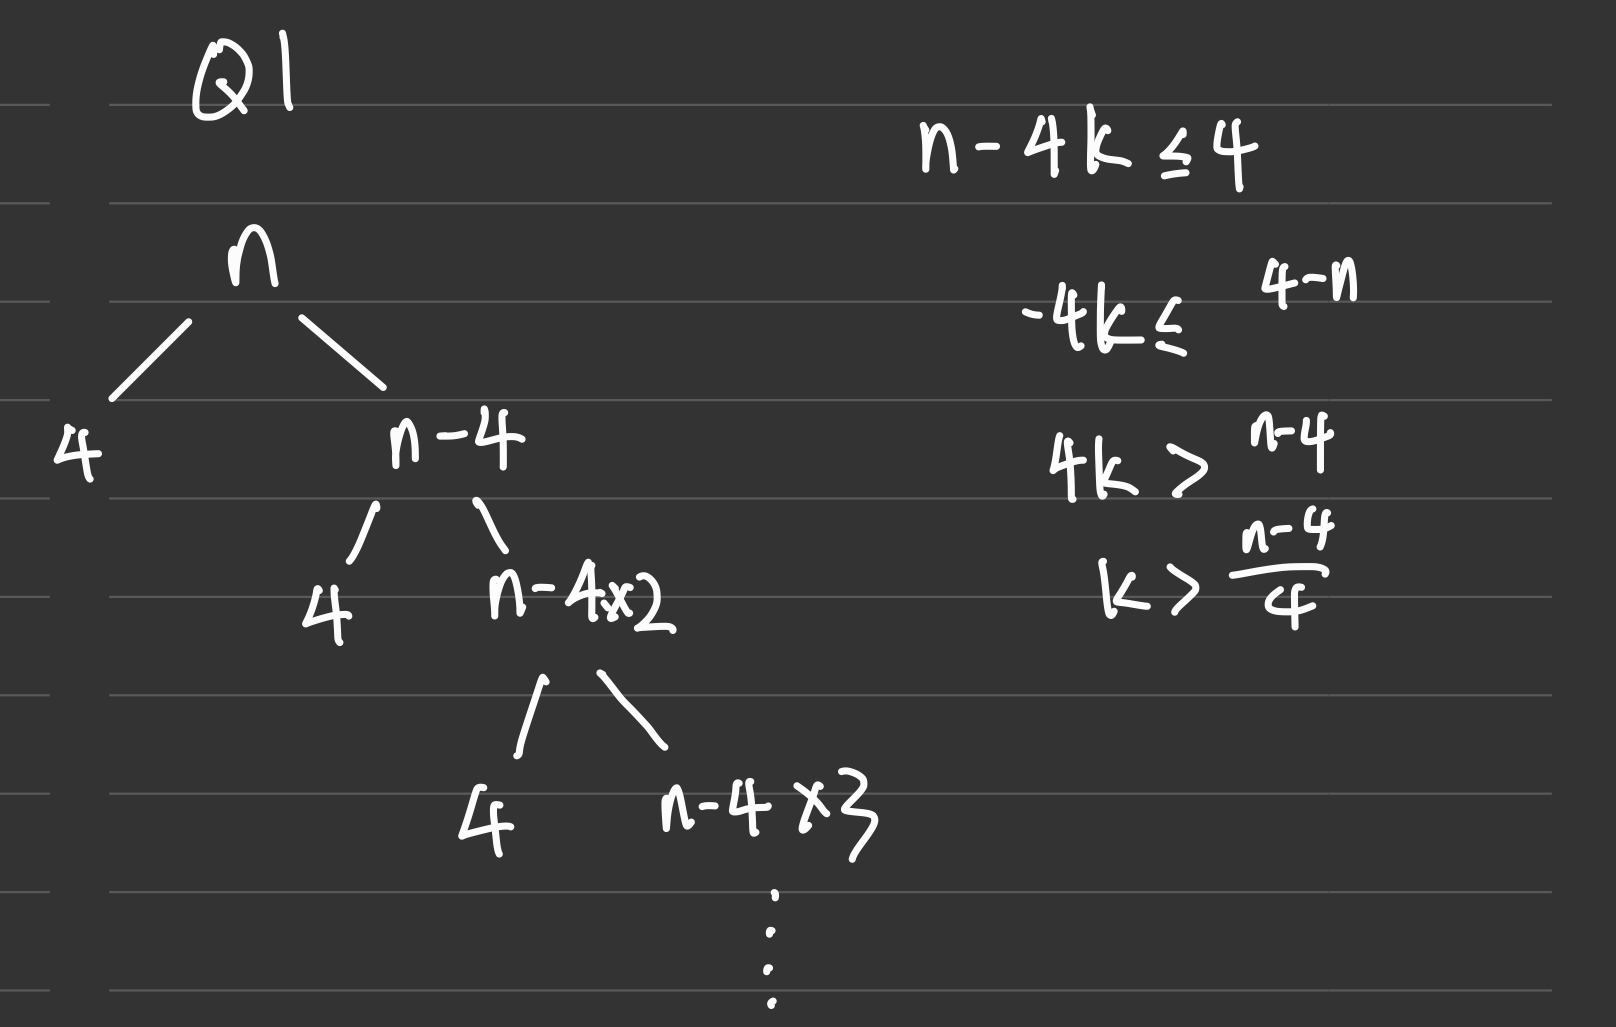
\includegraphics[width=0.7\textwidth]{HW6_Q1(a).PNG}
\end{center}

\begin{align*}
T(n) = \begin{cases}
\Theta(1)& : n \leq 4.\\
T(n-4) + T(4) +\Theta(n)& : n > 4 
\end{cases}
\end{align*}


\textbf{Finding the depth of tree first}
\begin{align*}
n-4k & \leq 4\\
-4k &\leq 4-n \\
4k &> n-4\\
k &>\ceil{ \frac{n-4}{4}}\\
k &\approx   \frac{n-4}{4}
\end{align*}

\textbf{Total run time complexity:\\}
\begin{align*}
\frac{n-4}{4} \cdot n &= \frac{n^2-4n}{4}\\
\end{align*}

\textbf{Asymptotic Solution:\\}
\begin{align*}
\lim _{n\to \infty }\:\frac{\frac{n^2-4n}{4}}{n^2} &= \lim _{n\to \infty }\:\frac{2n-4}{8n}\\
&= 1/4
\end{align*}
\textbf{This modified Merge Sort Algorithm has tight bound as $\Theta(n^2)$}
\end{proof}

\newpage

\item \label{(b)}~Consider a modified Merge-Sort algorithm that at each recursion splits an array of size $n$  into two subarrays of sizes $\frac{1}{5}n$ and $\frac{4}{5}n$, respectively. Write down a recurrence relation for this modified Merge-Sort algorithm and give its asymptotic solution.


\begin{proof}[Answer]
% YOUR ANSWER HERE
\begin{center}
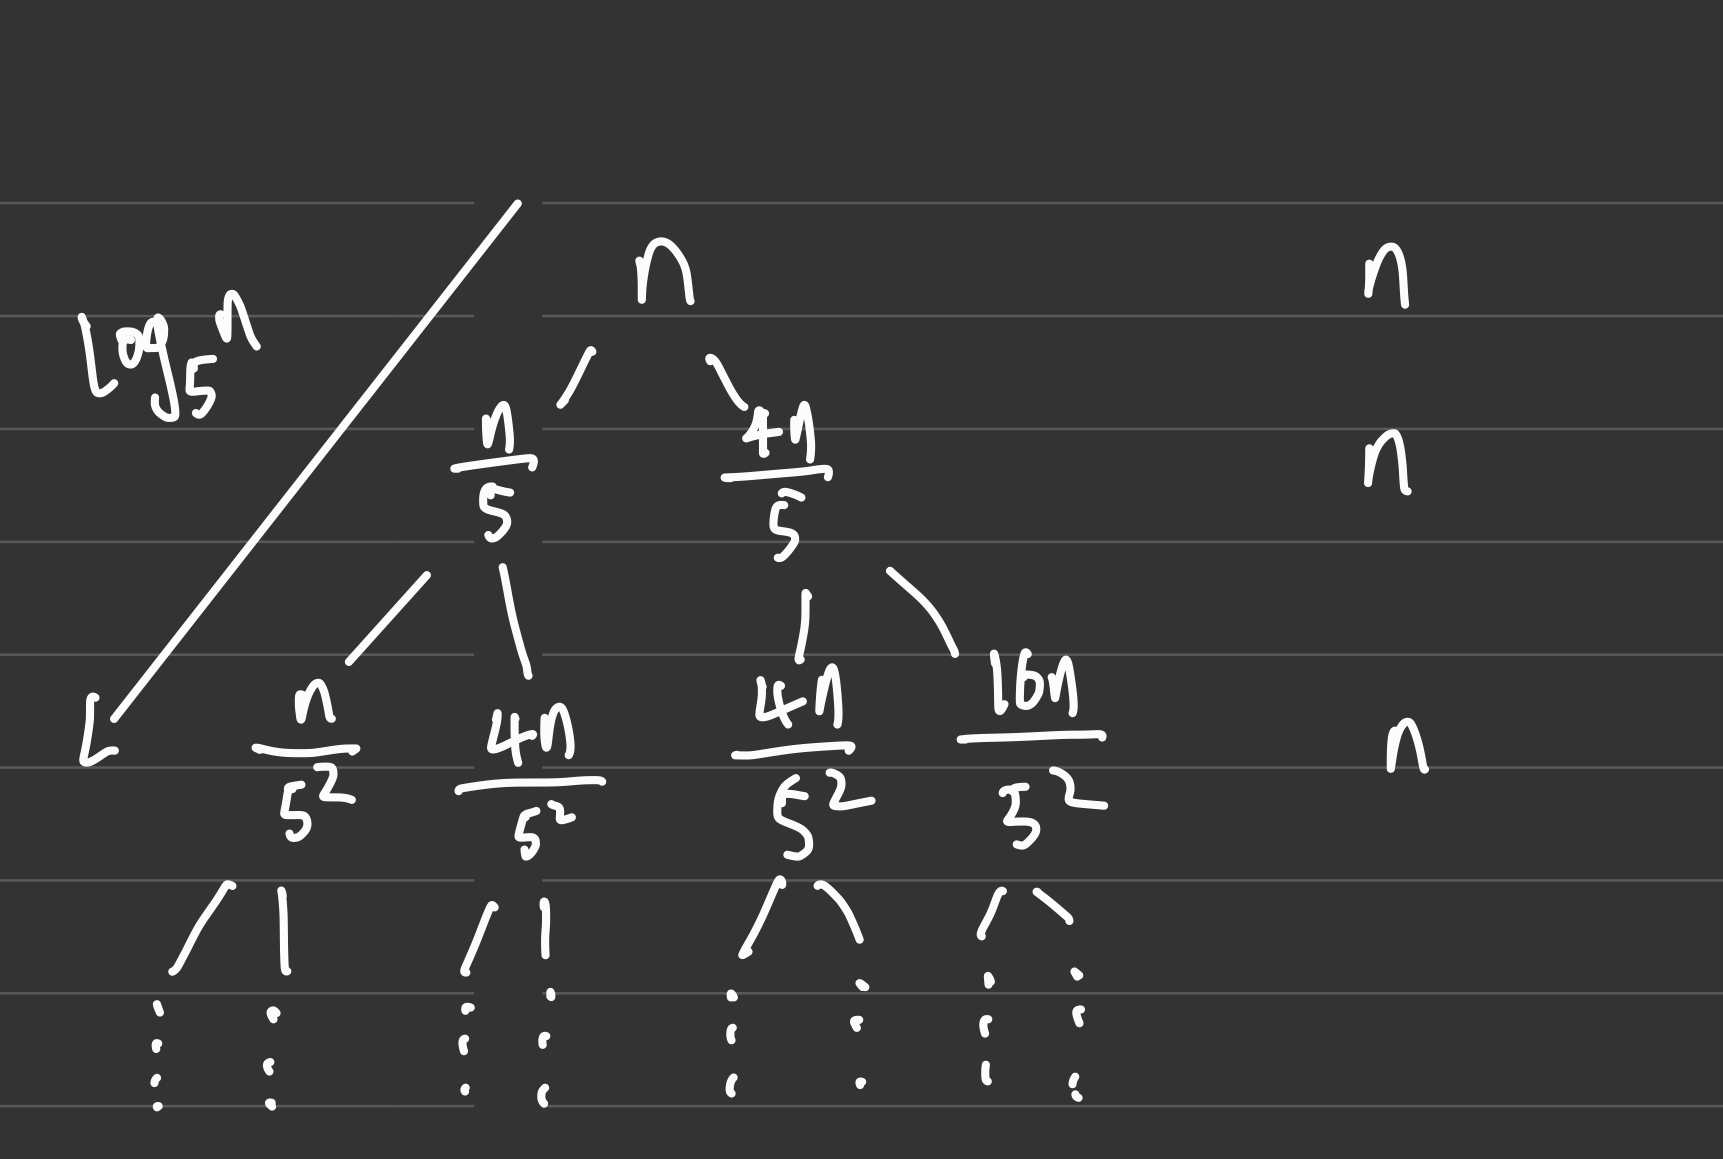
\includegraphics[width=0.7\textwidth]{HW6_Q1(b).PNG}
\end{center}

\begin{align*}
T(n) = \begin{cases}
\Theta(1)& : n \leq 5.\\
T(\frac{n}{5}) + T(\frac{4n}{5}) +\Theta(n)& : n > 5
\end{cases}
\end{align*}


\textbf{Finding the depth of tree first}
\begin{align*}
\frac{n}{5^k} & \leq 5\\
\frac{n}{5} & \leq 5^k \\
log_5 \frac{n}{5} \leq k\\
k &\geq log_5 \frac{n}{5}\\
k &\approx   log_5 \frac{n}{5}
\end{align*}

\textbf{Total run time complexity:\\}
\begin{align*}
log_5 \frac{n}{5} \cdot n &= n log_5 \frac{n}{5}\\
\end{align*}

\textbf{Asymptotic Solution:\\}
\begin{align*}
\lim _{n\to \infty }\:\frac{nlog_5\left(\frac{n}{5}\right)}{nlog_5\left(n\right)} &= \lim _{n\to \infty }\:\frac{\frac{1}{ln\left(5\right)\left(\frac{n}{5}\right)}}{\frac{1}{ln\left(5\right)\left(n\right)}}\\
&= \lim _{n\to \infty }\:\frac{ln\left(5\right)n}{ln\left(5\right)\left(\frac{n}{5}\right)}\\
&= 5
\end{align*}
\textbf{This modified Merge Sort Algorithm has tight bound as $\Theta(nlog_5\left(n\right))$}
\end{proof}


\newpage

\item \label{(c)}~Suppose that we modify the Merge-Sort algorithm in such a way that on alternating levels of the recursion, the partitioning is either a $(2, n-2)$ split or a $(n/2,~n/2)$ split. Write down a recurrence relation for this modified Merge-Sort algorithm and give its asymptotic solution. Then, give a verbal explanation of how this Merge-Sort algorithm changes the running time of Merge-Sort.


\begin{proof}[Answer]
% YOUR ANSWER HERE
\begin{center}
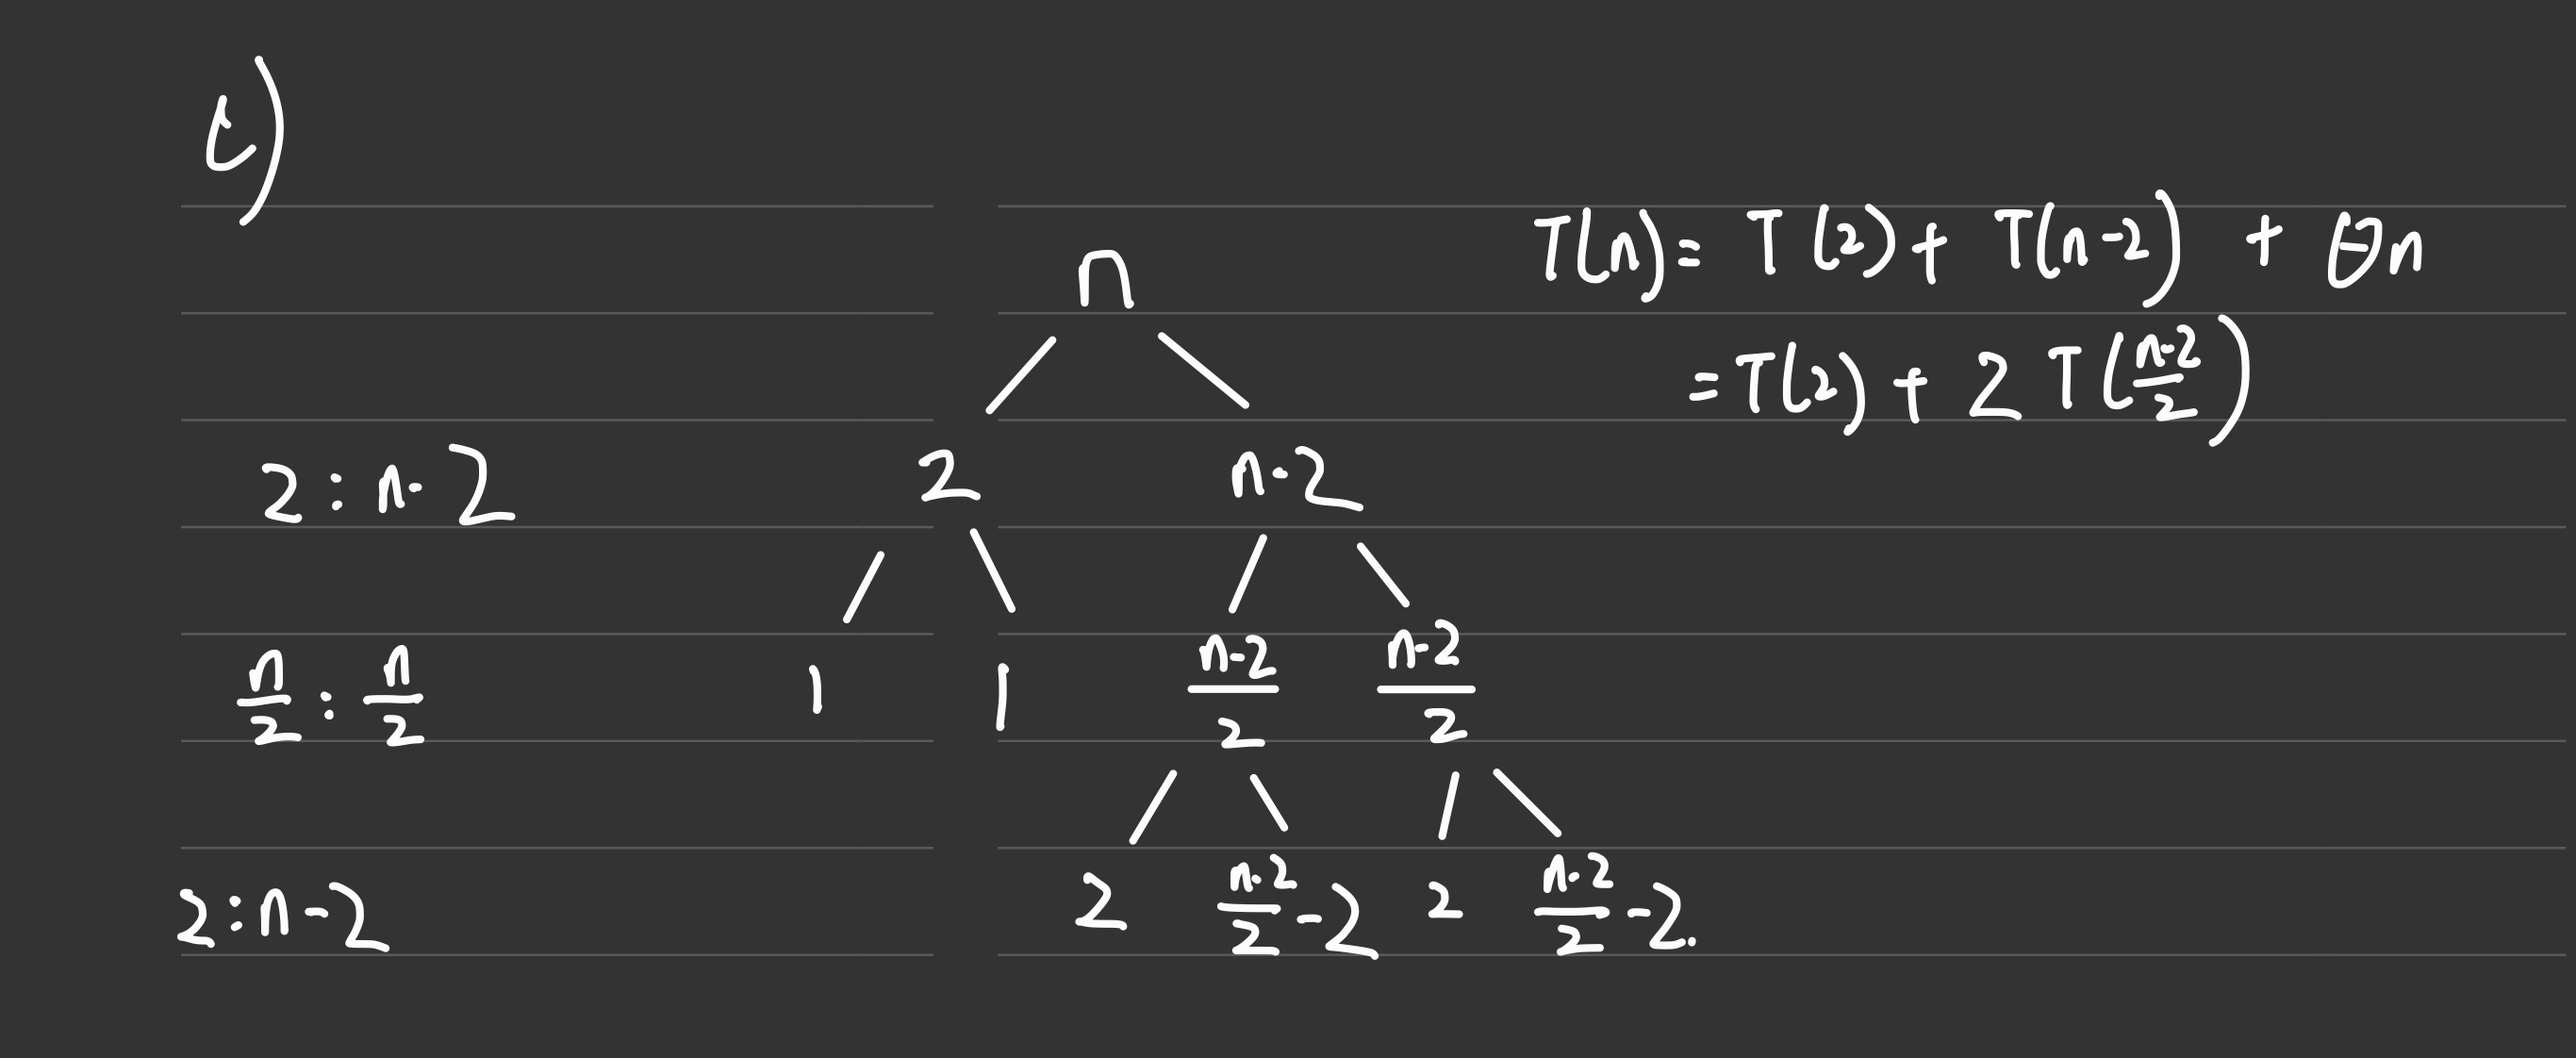
\includegraphics[width=0.7\textwidth]{HW6_Q1(c).PNG}
\end{center}


\begin{align*}
T_{(2,n-2)}(n) = \begin{cases}
\Theta(n)& : n \leq 2.\\
T(2) + T(n-2) +\Theta(n)& : n > 2 
\end{cases}
\end{align*}

\begin{align*}
T_{(n/2,n/2)}(n) = \begin{cases}
\Theta(n)& : n \leq 2.\\
2T(\frac{n-2}{2}) + \Theta(n) & : n > 2 
\end{cases}
\end{align*}

\begin{align*}
T(n) &= T(2) + T(n-2) + \Theta(n)\\
&= T(2) + 2T(\frac{n-2}{2}) +2\Theta(n)
\end{align*}

\textbf{For finding the asymptotic solution, we could ignore the term T(2) and left with $2T(\frac{n-2}{2}).$}
\textbf{Finding the depth of tree first}
\begin{align*}
\frac{n-2}{2^{0.5k}} & \leq 2\\
n-2 &< 2^{0.5k+1}\\
log_2\left(n-2\right) &\leq (0.5k+1)\\
k &\geq 2 (log_2\left(n-2\right)-1)\\
k &\approx   2 (log_2\left(n-2\right)-1)
\end{align*}

\textbf{Total run time is:\\}
\begin{align*}
2 (log_2\left(n-2\right)-1) \cdot n
\end{align*}

\textbf{Asymptotic Solution is:\\}
\begin{align*}
2 (log_2\left(n-2\right)-1) \cdot n \in  \Theta(nlog_2(n))
\end{align*}

\textbf{This algorithm doesn't change the run time of Merge Sort a lot since they have the same tight bound as $nlog_2(n)$. But it does increase the run time by factor of 2 due to an extra level with (2,n-2) splitting in each original algorithm level if we focus on the details of run time of this modified merge sort algorithm.\\}
\textbf{In this algorithm, the size of array will reduce whenever its recurrence has $T_{(n/2,n/2)}(n)$  at the layer $(n/2,n/2)$, and then the depth of tree will go further down. But, when its recurrence is $T_{(2,n-2)}(n)$, the depth of tree will not go further down and it delays the run-time of whole algorithm. And the factor of 2, I mentioned above, comes from this recurrence. }
\end{proof}

\end{enumerate}
\end{required}


\newpage
\section{Standard 18: Quicksort.}

\subsection{Problem 2}
\begin{required}
Given an input array $\{3,~7,~1,~8,~2,~6,~5,~4\}$. Consider the deterministic QuickSort algorithm and show the input array, the output array, and the global array at every partition as in the example in Section 2.1.1 of the course notes for week 8 (see Week 8 under ``Modules" of the course canvas). 

\begin{proof}[Answer]
% YOUR ANSWER HERE
\begin{center}
\begin{tabular}[c]{|c c c|c c c|} 
	Procedure& arguments& input&output &return&global array  \\\hline
	first & x=4 p=0 r=7& A=$[3,~7,~1,~8,~2,~6,~5,~\textbf{4}]$ &$[3, 1, 2 \mid  \textbf{4} \mid 7, 6, 5, 8 ]$&r = 3& $[3, 1, 2, 4, 7, 6, 5, 8 ]$\\
	L QS&x=2 p=0,r=2& A= $[3,1,\textbf{2}]$ & $ [1,\textbf{2},3]$ &r = 1& $[1, 2, 3, 4, 7, 6, 5, 8]$\\
	R QS&x=8 p=4,r=7& A= $[7,6,5,\textbf{8}]$ &$[7,6,5,\textbf{8}] $&r = 7&$[1, 2, 3, 4, 7, 6, 5, 8]$\\
	L QS& x=5 p=4,r=6& A=$[7,6,\textbf{5}]$ & $[\textbf{5}, 6,7]$ &r = 5& $[1, 2, 3, 4, 5, 6, 7, 8]$\\
	R QS& x=8 p=8,r=7(violated)& A = $[8]$& $N/A$ &r = NA& $[1, 2, 3, 4, 5, 6, 7, 8]$\\
\end{tabular}
\end{center}	
\end{proof}

\end{required}

\newpage
\subsection{Problem 3}
\begin{required}

Suppose that we modify {\sc Partition}($A,s,e$) so that it chooses the median element of $A[s..e]$ in calls that occur in nodes of even depth of the recursion tree of a call {\sc Quicksort}($A[1, \ldots, n],1, n$), and it chooses the minimum element of $A[s..e]$ in calls that occur in nodes of odd depth of this recursion tree. \\
  
\noindent Assume that the running time of this modified {\sc Partition} is still $\Theta(n)$ on any subarray of length $n$. You may assume that the root of a recursion tree starts at level $0$ (which is an even number), its children are at level 1, etc. \\
  
\noindent Write down a recurrence relation for the running time of this version of {\sc Quicksort} given an array $n$ distinct elements and solve it asymptotically, i.e.\ give your answer as $\Theta(f(n))$ for some function $f(n)$. Show your work.

\begin{proof}[Answer]
% YOUR ANSWER HERE
\begin{center}
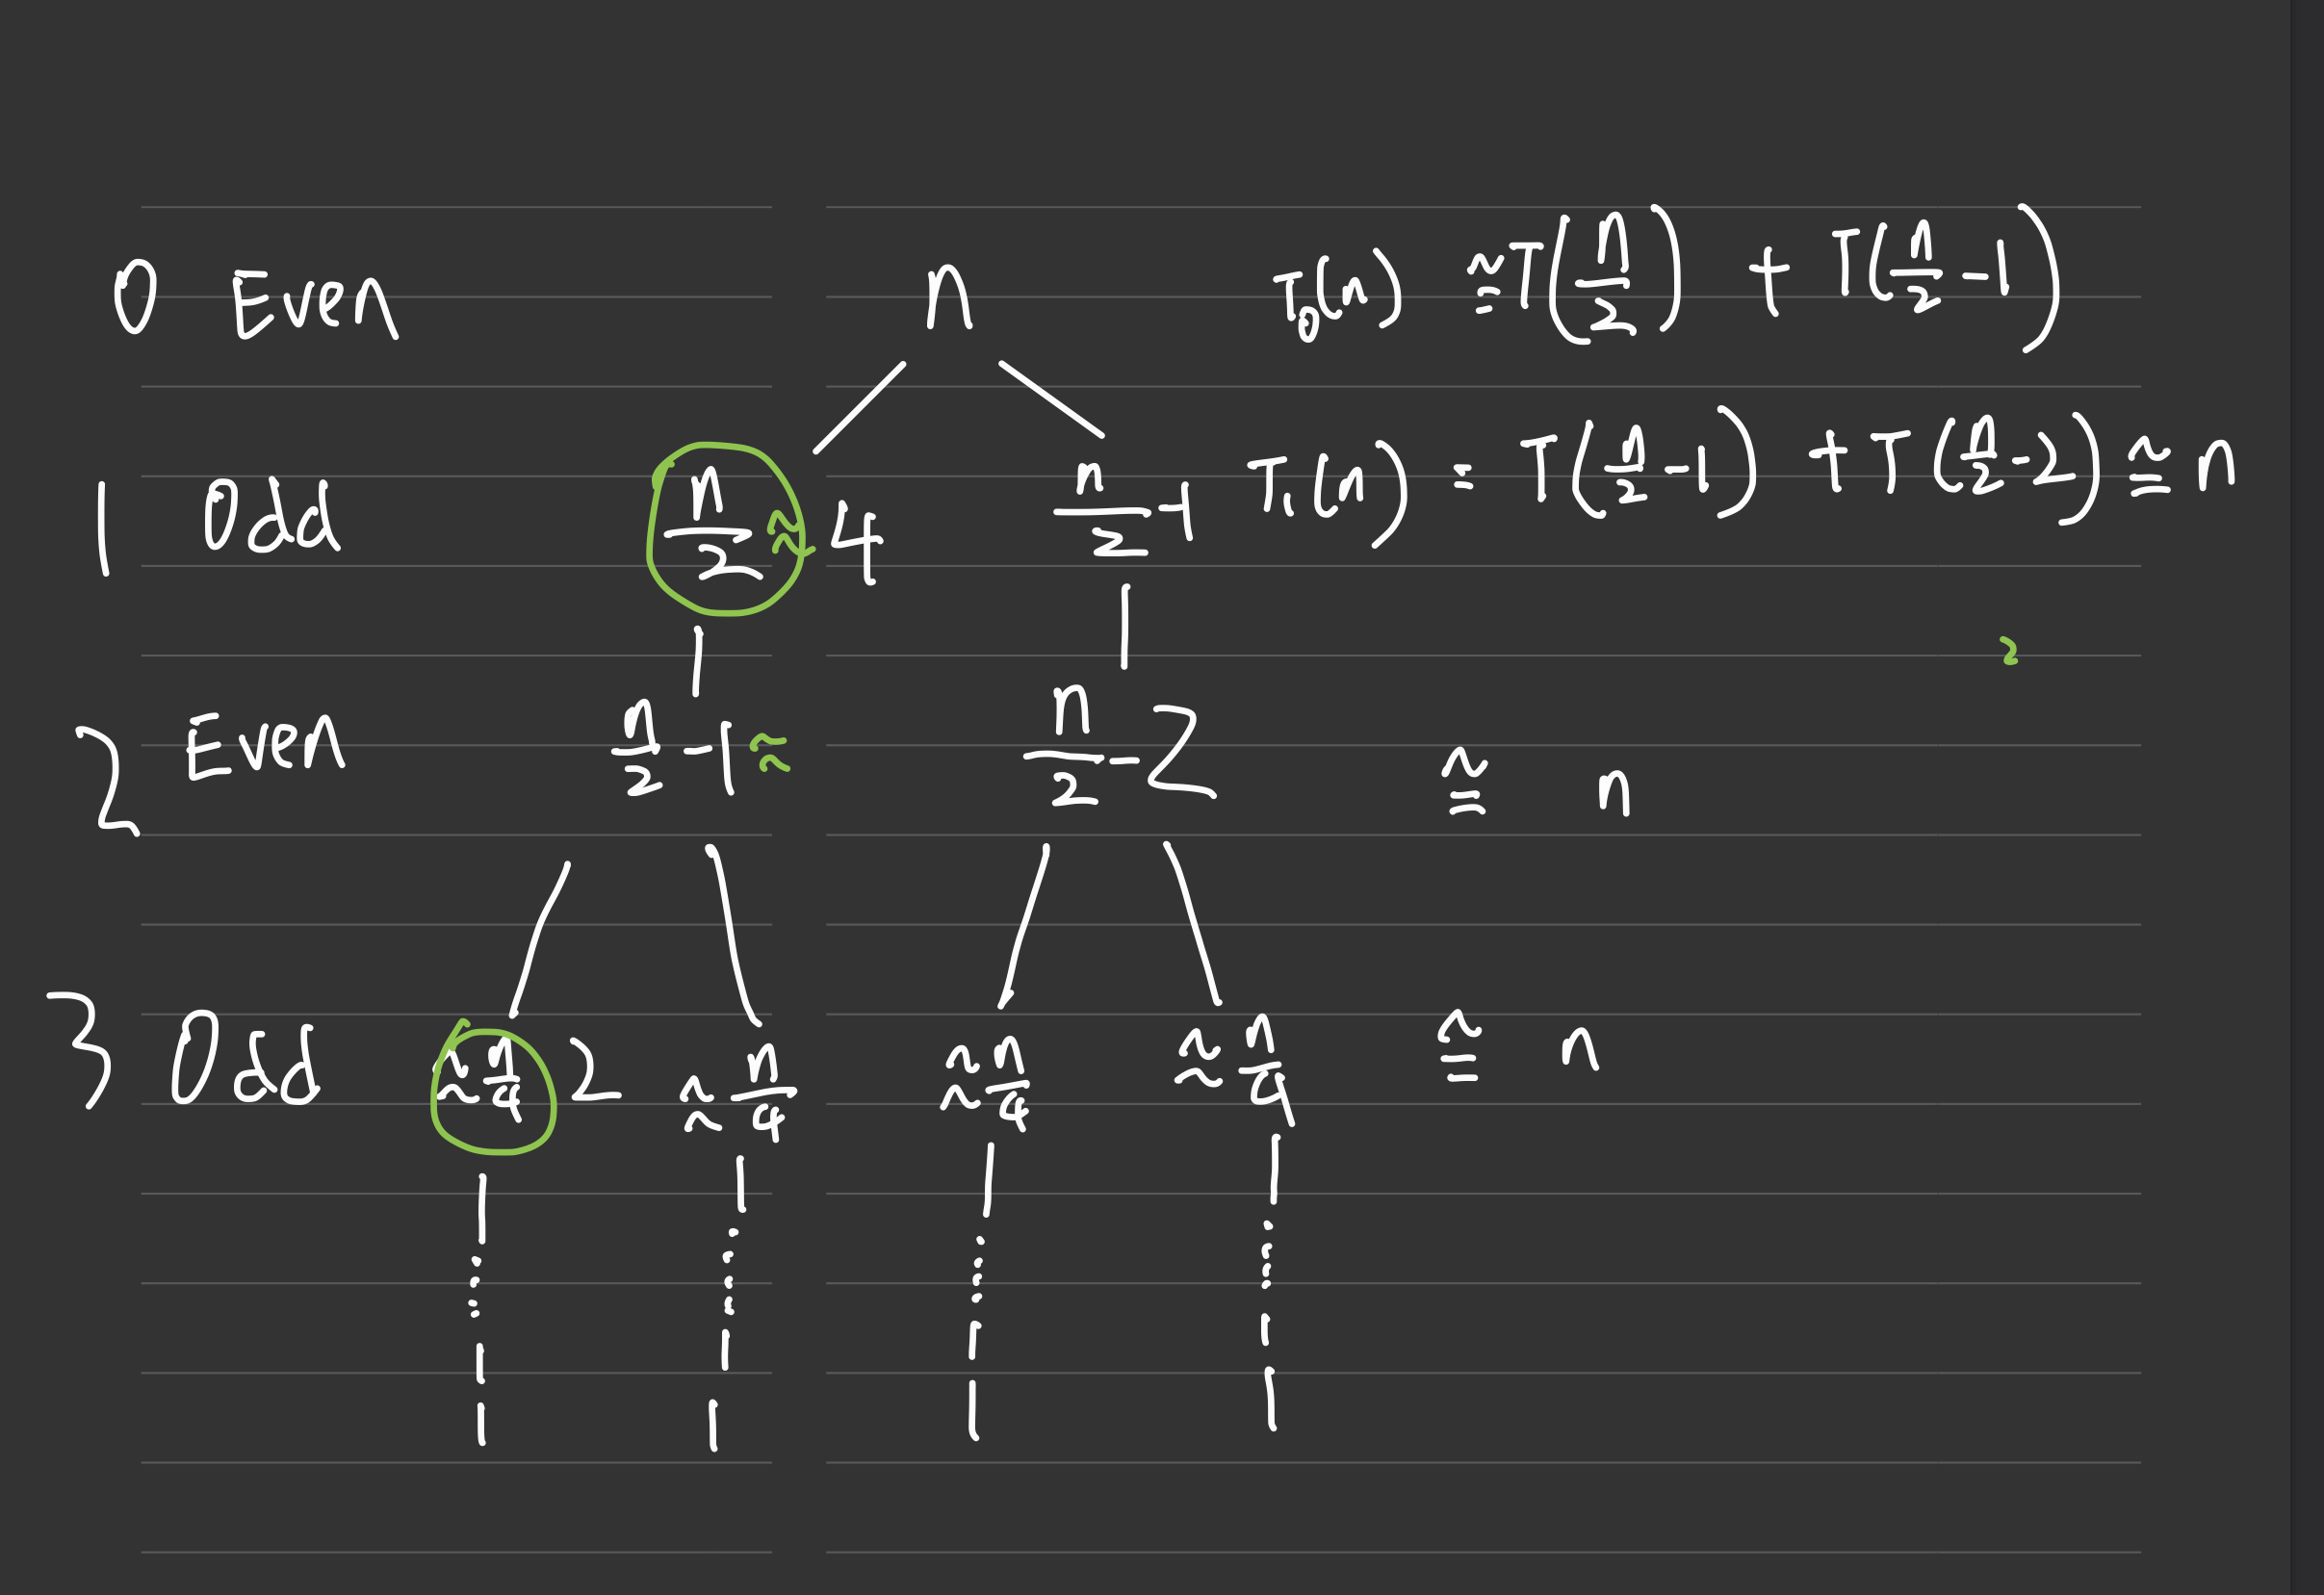
\includegraphics[width=0.7\textwidth]{HW6_Q3.PNG}
\end{center}

\textbf{ Above is my general idea about what's going on in this algorithm.\\}
\begin{align*}
T_{even}(n) = \begin{cases}
\Theta(n)& : n \leq 1.\\
T(\frac{n}{2}) + T(\frac{n}{2}-1) +\Theta(n)& : n > 1 
\end{cases}
\end{align*}

\begin{align*}
T_{odd}(n) = \begin{cases}
\Theta(n)& : n \leq 1.\\
T(n-1) + \Theta(n) & : n > 1 
\end{cases}
\end{align*}

\begin{align*}
T(n) &= T(\frac{n}{2}) + T(\frac{n}{2} -1 ) + \Theta(n)\\
&= T(\frac{n}{2} -1 ) +T(\frac{n}{2} -2 ) + \Theta(n)\\
&= .....
\end{align*}

\textbf{Finding the depth of tree first}
\begin{align*}
\frac{n}{2^{0.5k}} & \leq 1\\
n &< 2^{0.5k}\\
log_2\left(n\right) &\leq (0.5k)\\
k &\geq 2 log_2\left(n\right)\\
k &\approx   2 log_2\left(n\right)
\end{align*}

\textbf{At each level, I approximate the expression (i.e. ignoring the constant part). As seen in level 1, there are two nodes. So the total run time complexity at this level is $2 \cdot \frac{n}{2} = n$\\
And as seen in level 2, 3...,  Run time complexity at each level approximately equal to n.\\}
\textbf{Total run time complexity is:\\}
\begin{align*}
2 log_2\left(n\right) \cdot n &= 2n log_2\left(n\right)\\
\end{align*}
\textbf{Tight bound:\\}
\begin{align*}
\lim _{n\to \infty }\left(\frac{2nlog_2\left(n\right)}{nlog_2\left(n\right)}\right) &= 2
\end{align*}
\textbf{This algorithm has bound as $\Theta(nlog_2\left(n\right))$}
\end{proof}

\end{required}

\end{document} % NOTHING AFTER THIS LINE IS PART OF THE DOCUMENT